\documentclass{article} 
\usepackage{xcolor}
\usepackage{float}
\usepackage{graphicx}
\usepackage{caption}
\usepackage{subcaption}
\linespread{1}
\usepackage[utf8]{inputenc} 
\usepackage[T1]{fontenc}
\usepackage{enumitem}
\usepackage{amsmath}
\usepackage{mathtools}
\usepackage{hyperref}

\author{Luca Corbucci}
\title{Machine Learning Exercise Sheet 05}
\begin{document}
\maketitle

\textbf{Problem 1}
\newline

a) The posterior distribution $p(y|x)$ is a Bernoulli Distribution because we are reasoning about the variable $y$ which is a variable that has only 2 possible values, $0$ and $1$.

b) We know that: $$P(y=1|x) = \frac{P(x|y=1)P(y=1)}{P(x|y=1)P(y=1) + P(x|y=0)P(y=0)} =$$ 
$$ = \frac{expo(x|\lambda_1)\frac{1}{2}}{\frac{1}{2}expo(x|\lambda_0) + \frac{1}{2}expo(x|\lambda_0)} = 1 + \frac{\lambda_1e^{-\lambda_1x}}{\lambda_0e^{-\lambda_0x}}$$ $$=\frac{1}{1+exp(-a)}$$

Where $a=ln\frac{\lambda_1e^{-\lambda_1x}}{\lambda_0e^{-\lambda_0x}}$

The values of $x$ that are classified as class 1 are the ones for which holds $a>0$:

$$ln\frac{\lambda_1e^{-\lambda_1x}}{\lambda_0e^{-\lambda_0x}} > 0$$
$$ln(\lambda_1) + ln(e^{-\lambda_1x}) - ln(\lambda_0) - ln(e^{-\lambda_0x}) > 0$$
$$ln(\lambda_1) - \lambda_1x - ln(\lambda_0) + \lambda_0x > 0$$
$$x(\lambda_0 - \lambda_1) > ln(\lambda_0) - ln(\lambda_1)$$
$$x>ln(\frac{\lambda_0}{\lambda_1})\frac{1}{\lambda_0-\lambda_1}$$
\newline

\textbf{Problem 2}
\newline

a) If the dataset is linearly separable we have for each data point $x_i$:

$$w^Tx_i > 0$$

or 

$$w^Tx_i < 0$$

The MLE solution occurs when $\sigma = \frac{1}{2}$ and the hyperplane $w^Tx = 0$ separates the two classes.
The magnitude of $w$ goes to infinity in this case.

b) The problem is that if we use a dataset that is linerly separable MLE leads to overfitting.
A possible solution for this problem is the usage of the weights regularization.
In this case the loss function is $$E(w) = -ln \ p(y|w,x)+\lambda	 ||w||^2_q$$

Another possible solution: we can compute the prior probability and then the MAP, in this way we can solve the overfitting problem.
\newline

\textbf{Problem 3}
\newline

We define the softmax as:
$$\sigma(x)_i = \frac{exp(x_i)}{\sum_{k=1}^k exp(x_k)}$$

To show that is equal to the sigmod in the 2-class case I consider the $P(y_i = x_1)$ where the $y_i$ is the prediction and $x_1$ is the predicted class.

$$P(y_1 = x_1) = \frac{exp(x_1)}{exp(x_1) + exp(x_2)} = 1 + \frac{exp(x_1)}{exp(x_2)}= 1 + exp(x_1 - x_2) = \frac{1}{1+exp(x2-x1)}$$

If $a = ln(x_1-x_2)$ we obtain:
$$\frac{1}{1+exp(-a)}$$

\textbf{Problem 4}
\newline

The basis function that makes the data linearly separable is:\begin{align}
    \phi(x_1,x_2) &= \begin{bmatrix}
           x_1 \\
           x_2 \\
           |x_1 + x_2|
         \end{bmatrix}
  \end{align}

I've plotted the original data and new generated data to check if they are linearly separable:

\begin{figure}[H]
\centering
  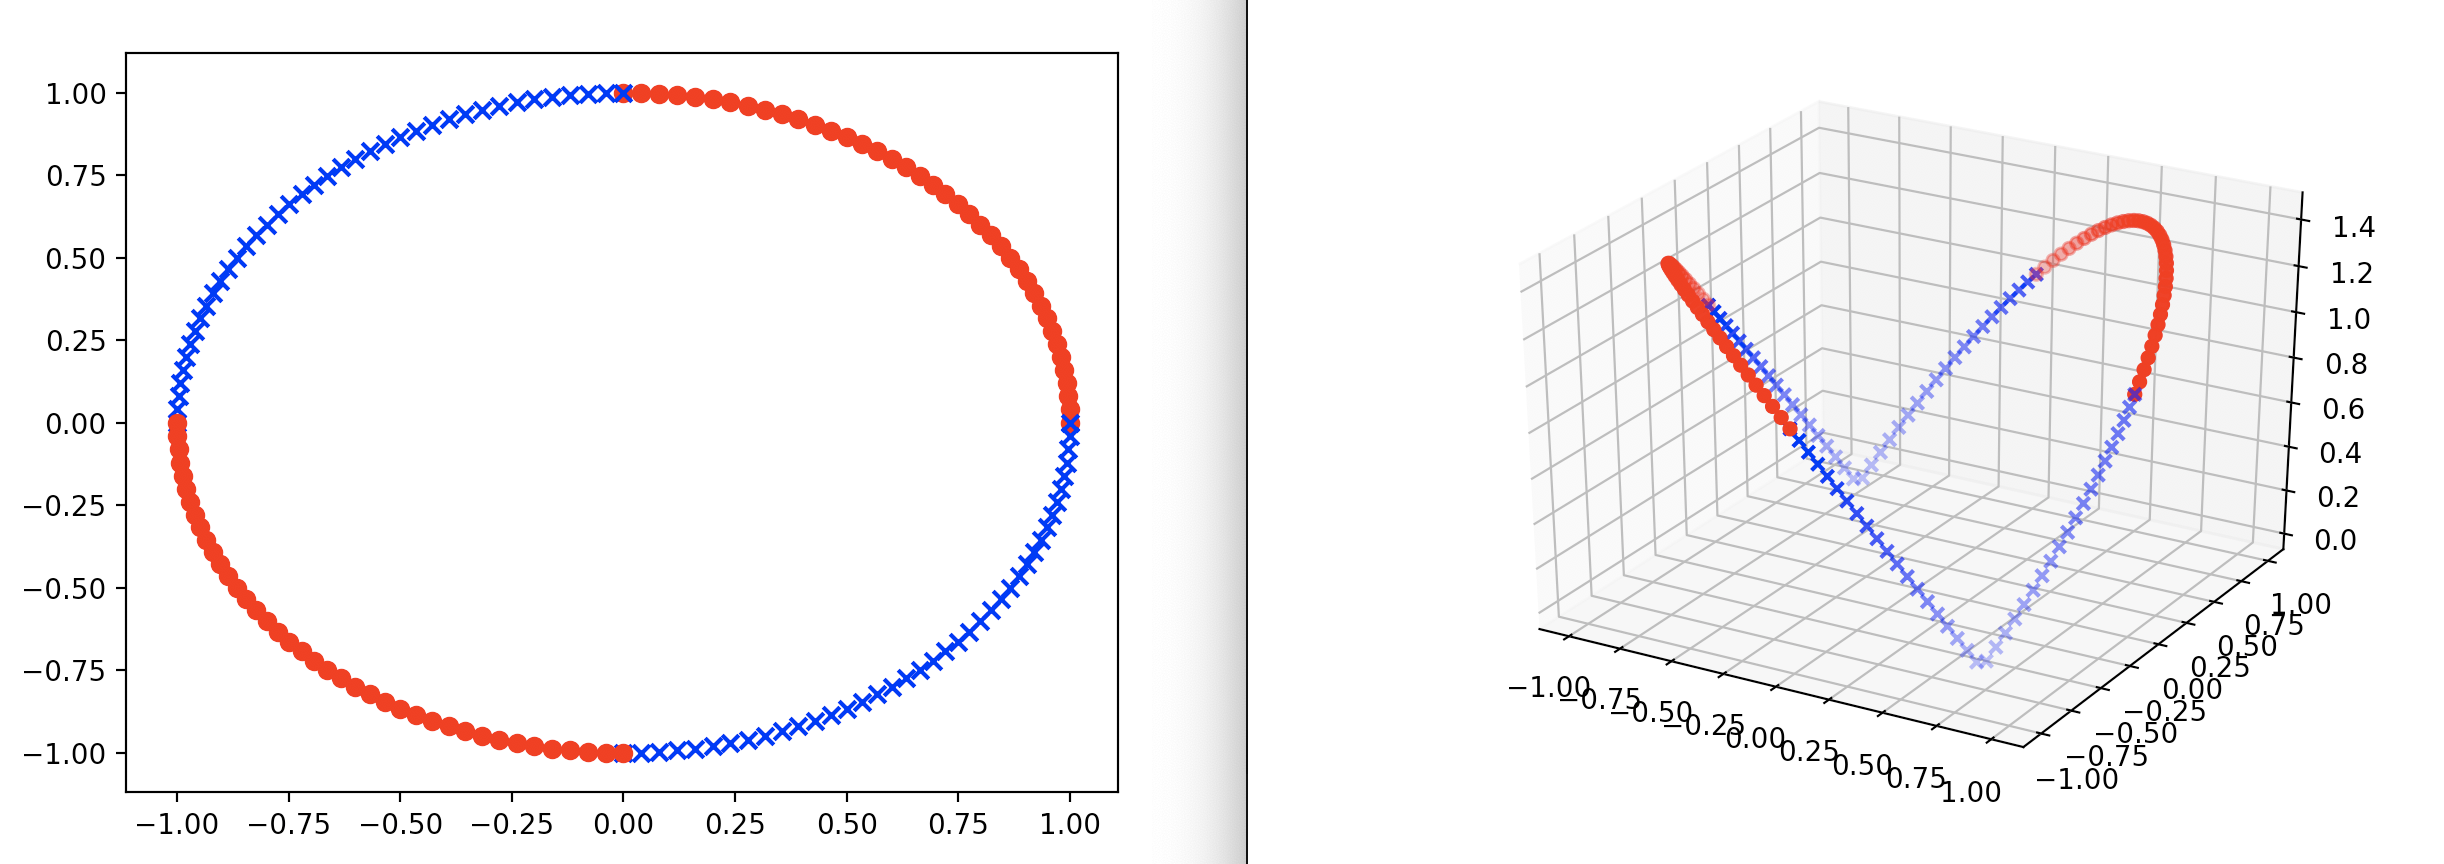
\includegraphics[width=\linewidth]{Exercise4.png}
\end{figure}

\end{document}